\documentclass[aspectratio=1610]{beamer}

\usepackage[ngerman]{babel}
\usepackage[utf8]{inputenc}
\usepackage[absolute,overlay]{textpos}
\usepackage{xcolor}
\usetheme{CambridgeUS}

\AtBeginSection[]
{
   \begin{frame}
       \frametitle{Outline}
       \tableofcontents[currentsection]
   \end{frame}
}

\title{Das \\„wer, wie, was, warum?“ \\der Verschlüsselung}

\author[Mic]{Mic \flq nomaster@chaosdorf.de\frq}

\institute[chaosdorf]{Chaos Computer Club Düsseldorf / Chaosdorf e.V.}

\date[]{8. September 2013}

\renewcommand{\quote}[2]
{
  \begin{exampleblock}{}
    {\large “#1”}
    \vskip5mm
    \hspace*\fill{\small--- #2}
  \end{exampleblock}
}


\begin{document}

  \begin{frame}
    \titlepage
  \end{frame}

  \begin{frame}{CryptoParty}
    \begin{itemize}
      \item
        Wir möchten den Menschen den praktischen Nutzen von Kryptographie erklären\\
        und ihnen bei der Installation der Programme auf ihren eigenen Geräten helfen.
    \pause
      \item
        Wir hoffen, dass sie durch eigenständiges Handeln\\
        den Nutzen und die Wichtigkeit von Kryptographie verstehen.
    \pause
      \item
        CryptoParties finden weltweit selbstorganisiert statt.\\
        Dabei sollen sie unabhängig und kostenlos bleiben.
    \end{itemize}
  \end{frame}

  \begin{frame}{Zitat}
    \quote{Man is least himself when he talks in his own person.\\
      Give him a mask, and he will tell you the truth.}
      {Oscar Wilde}
  \end{frame}
  \begin{frame}{Manifest}
    \begin{enumerate}
      \pause
      \item Wir alle sind die User.
      \pause
      \item Privatsphäre ist Menschenrecht.
      \pause
      \item Privatsphäre ist ein Recht des Individuums.
      \pause
      \item Privatsphäre ist Hoheit des Individuums.
      \pause
      \item Alle Menschen ist dieses Recht zuteil.
      \pause
      \item Kryptographie ist für alle da.
      \pause
      \item Überwachung und Zensur sind untrennbar. Maschinen sollen dazu nicht dienen.
      \pause
      \item Programmcode ist Sprache und unterliegt dem Recht auf freie Meinungsäußerung.
      \pause
      \item Die Feinde der Kryptographie wären im 15. Jahrhundert die Feinde der Pressefreihet gewesen.
    \end{enumerate}
  \end{frame}

  \begin{frame}{Privatsphäre}
    Privatsphäre ist…
    \begin{itemize}
      \pause
      \item Der Bereich der persönlichen Freiheit
      \pause
      \item Das Recht, in Ruhe gelassen zu werden
      \pause
      \item Persönliche Daten, deren Verbreitung das Individuum kontrolliert
    \end{itemize}
  \end{frame}

  \begin{frame}{Warum kämpfen?}
    “Ich habe doch nichts zu verbergen.”
    \begin{itemize}
      \item Unbewusste Geheimnisse
      \item Unsichere Zukunft
      \item Auswirkungen auf andere
      \item Chilling Effect
    \end{itemize}
  \end{frame}

  \begin{frame}{Die Lösung}
    \begin{columns}
      \begin{column}{.5\textwidth}
        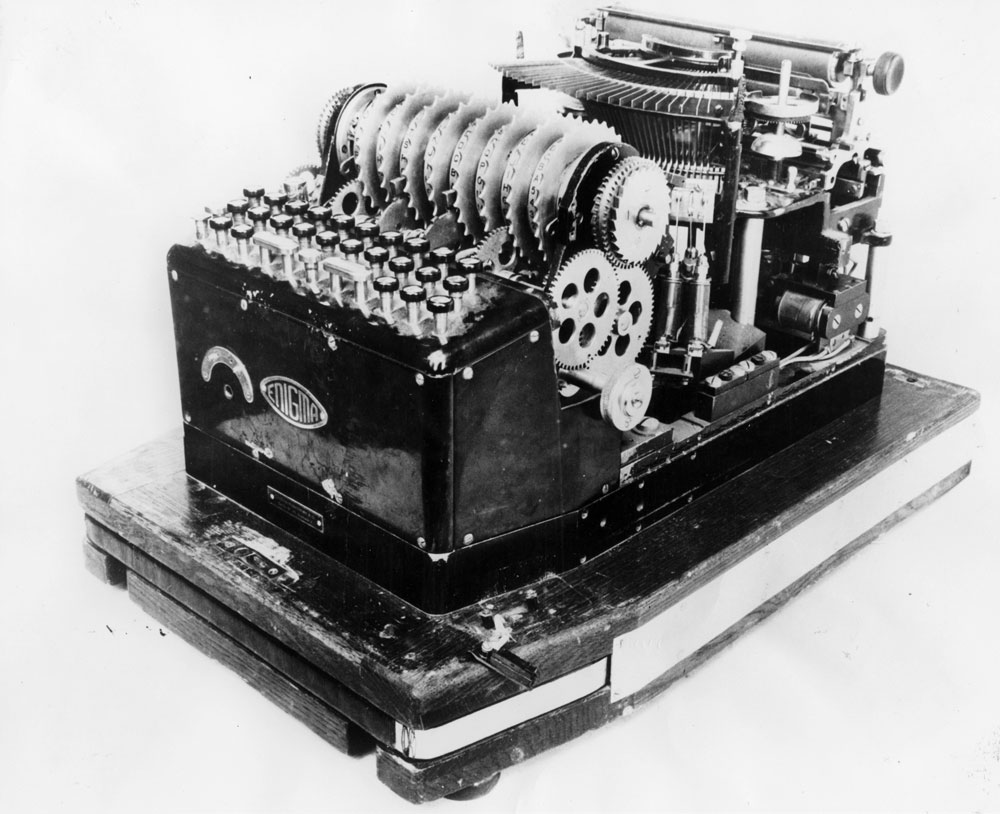
\includegraphics[width=\textwidth]{enigma.jpg}
      \end{column}
      \begin{column}{.5\textwidth}
        \begin{itemize}
          \pause
          \item Kryptographie verbirgt Informationen vor der Öffentlichkeit
          \pause
          \item Das Geheimnis muss bekannt sein
          \pause
          \item Ohne Vertrauen läuft es nicht
        \end{itemize}
      \end{column}
    \end{columns}
  \end{frame}

  \begin{frame}{Vertrauen}
    “Traue niemandem!” --- anonymous
    \begin{itemize}
      \pause
      \item Autoritäten sind an ihrem Ende
      \pause
      \item Wir bilden individuelle Vertrauensverhältnisse
      \pause
      \item Ein Netz des Vertrauens entsteht
      \pause
      \item (Tele-)Kommunikation als erweiterte Privatsphäre
    \end{itemize}
  \end{frame}

  \begin{frame}{Identität}
    “Man kann nicht zweimal in den selben Fluss steigen” --- panta rhei
    \begin{itemize}
      \pause
      \item Menschen ändern sich
      \pause
      \item Schlüssel ändern sich
      \pause
      \item Vertrauen heißt die Autonomie des Anderen anzuerkennen
      \pause
      \item Vertrauen heißt auch, die Verschwiegenheit des Anderen anzunehmen
      \pause
      \item Vertrauen entsteht über die Zeit
    \end{itemize}
  \end{frame}

  \begin{frame}{Schlüssel}
    \begin{columns}
      \begin{column}{.5\textwidth}
        
\includegraphics[width=\textwidth]{security.jpg}
      \end{column}
      \begin{column}{.5\textwidth}
        \begin{itemize}
          \pause
          \item Symmetrische Schlüssel für Datenträger
          \pause
          \item Asymmetrische Schlüssel für Telekommunikation
          \pause
          \item Verschlüsselung ist ein Protokoll
        \end{itemize}
      \end{column}
    \end{columns}
  \end{frame}

  \begin{frame}{Meta}
    Nun kommt die Enttäuschung
    \begin{itemize}
      \pause
      \item Verschlüsselung versteckt nur die Nachricht, nicht den Umschlag
      \pause
      \item Die Metadaten bleiben öffentlich
        \begin{itemize}
          \pause
          \item Identität der Sender und Empfänger
          \pause
          \item Zeitpunkt und Zugangspunkt
          \pause
          \item Länge und Medium
        \end{itemize}
    \end{itemize}
  \end{frame}

  \begin{frame}{Anonymität}
    \begin{columns}
      \begin{column}{.5\textwidth}
        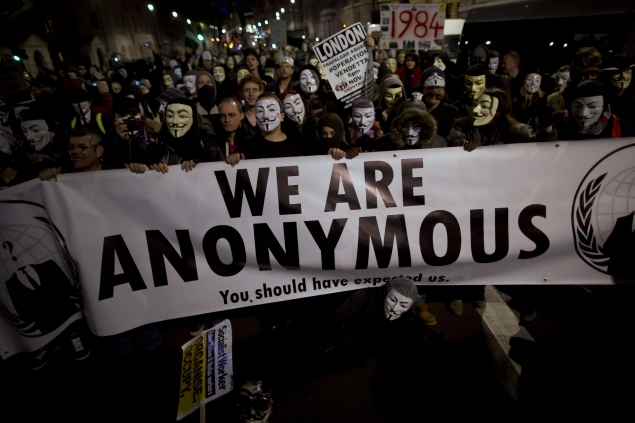
\includegraphics[width=\textwidth]{anonymous.jpg}
      \end{column}
      \begin{column}{.5\textwidth}
        \begin{itemize}
          \pause
          \item Hinreichend verschleierte Identität
          \pause
          \item Temporäre, vom Körper getrennte Identität
          \pause
          \item Black Bloc als möglichst großer, aber eingeschränkter Personenkreis
          \pause
          \item sie auch: Pseudonymität, Autonymität
        \end{itemize}
      \end{column}
    \end{columns}
  \end{frame}

  \begin{frame}{Sicherheit}
    \quote{Ein System muss auch dann sicher sein,\\wenn das gesamte System offen liegt,\\ausgenommen des Geheimnisses.}{Kerckhoff’sches Prinzip}
    \begin{itemize}
      \pause
      \item Die Software muss einsehbar sein.
      \pause
      \item Der Transport kann öffentlich sein.
      \pause
      \item Keine Sicherheit durch Obskurität!
    \end{itemize}
  \end{frame}

  \begin{frame}{Werkzeuge}
    Freie Software für Kryptographie
    \begin{itemize}
      \pause
      \item Verschlüsselung von Datenträgern
      \begin{itemize}
        \pause
        \item TrueCrypt
        \pause
        \item LUKS (Linux)
      \end{itemize}
      \pause
      \item Verschlüsselung von E-Mails
      \begin{itemize}
        \pause
        \item GnuPG
        \pause
        \item mit Thunderbird und Enigmail
        \pause
        \item mit GPGTools und Apple Mail
        \pause
      \end{itemize}
      \pause
      \item Anonymisierung von Verbindungen
      \begin{itemize}
        \pause
        \item OpenVPN
        \pause
        \item Tor
      \end{itemize}
    \end{itemize}
  \end{frame}

  \begin{frame}{Dokumentation}
    Handbücher
    \begin{itemize}
      \pause
      \item CryptoParty Handbook \\ \url{http://www.cryptoparty.in/documentation/handbook}
      \pause
      \item Wikibooks Privacy-Handbuch \\ \url{https://de.wikibooks.org/wiki/Privacy-Handbuch}
    \end{itemize}
  \end{frame}

  \begin{frame}
    \center
    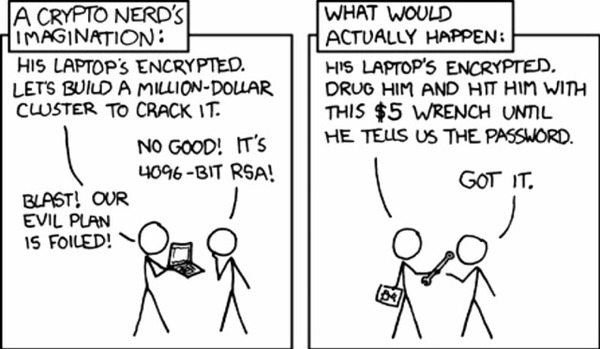
\includegraphics[width=.5\textwidth]{xkcd.jpg}
  \end{frame}

\end{document}
